\newpage
%--------------------------------------------------------------------------
%\section*{Entwurf}
\chapter{Design Patterns}
Entwurfsmuster sind Beschreibungen bewährter und erprobter Lösungen,
die als Vorlagen zur Lösung neuer Probleme
dienen können. Mit Hilfe von Musterkatalogen
kann so der Entwurf, die Wiederverwendung und Wartung von
Software vereinfacht werden.

\newslide
Beispiel\footnote{Design Patterns: Elements of Reusable Object-Oriented
  Software (Gamma, Helm, Johnson, Vlissides)}:
\begin{figure}[H]
\begin{center}
\includegraphics[width=0.7\linewidth]{uml/img/GoF}
\caption{Musterkatalog (Source: http://www.vincehuston.org/dp)}
\end{center}
\end{figure}
\newslide
\begin{itemize}
\item \underline{Erzeugungsmuster (Creational Patterns):}
  \begin{description}
  \item [factory method:] (FM) Erzeugung von Objekten
  \item [abstract factory:] (AF) Erzeugung unterschiedlicher Gruppen von Objekten
  \item [builder:] (BU) Einheitlicher Konstruktionsprozess komplexer Objekte
  \item [singleton:] (S) Sicherstellung, dass von einer Klasse nur eine
    einzige Instanz existiert
  \end{description}
\newslide
\item \underline{Strukturierungsmuster (Structural Patterns):}
  \begin{description}
  \item[adapter:](A) Konvertierung,Anpassung von Schnittstellen
  \item[bridge:] (BR) Entkopplung einer Schnittstelle (Abstraktion) von
    ihrer Implementation
  \item[composite:] (CP) Aufbau von Objektstrukturen (Stücklisten)
  \item[proxy:] (PX) Platzhalter zur Zugriffskontrolle eines Objektes
  \item[decorator:] (D) dynamisches Anhängen zusätzlicher Aufgaben an ein
    Objekt als Alternative zur Vererbung
  \item[facade:] (FA) Einheitliche Schnittstelle für den Zugriff auf
    unterschiedliche Schnittstellen von Subsystemen
  \end{description}
%\newslide
\newpage
\item \underline{Verhaltensmuster (Behavioral Patterns):}
  \begin{description}
  \item[observer:] (O) Abhängigkeitskontrolle zwischen Objekten, deren Zustand
   sich ändert und solchen
    die darüber informiert werden müssen
  \item[chain of responsibility:] (CR) Entkopplung von Sender und Empfänger,
    so dass mehrere Empfänger eine Anfrage behandeln können
  \item[mediator:] (MD) Kapselung der Interaktion von Objekten
  \item[iterator:] (IT) Sequentieller Zugriff auf die Elemente eines
     zusammengesetzten Objektes
  \item[command:] (CD) Kapselung einer Anfrage als Objekt
  \item[state:] (ST) Verhaltensänderung aufgrund von Zustandsänderungen
  \item[visitor:] (V) Ausführung von Funktionen auf einer Objektstruktur
  \end{description}
\end{itemize}
Weitere Infos:
\begin{itemize}
\item Wikipedia: \href{http://en.wikipedia.org/wiki/Design_Patterns}
   {en.wikipedia.org/wiki/Design\_Patterns}
 \item Vince Huston: \href{http://www.vincehuston.org/dp}
   {www.vincehuston.org/dp/}
\end{itemize}
 % Abstraktionen von Grundstrukturen:
%\begin{description}
%\item [Strategy:] allgemeine Schnittstelle zu mehreren Funktionsweisen
%\item [Decorator:] Ummantelung mit zusätzlichen Funktionen
%\item [Mediator:] Koordination zwischen Komponenten
%\item [Adapter:] Anpassung von Komponentenschnittstellen
%\item [Bridge:] Zugang zu unterschiedlich realisierten Komponenten mit ähnlicher
%  Funktionalität
%\item [Observer:] Überwachung und Reaktion auf Veränderungen
%\item [Proxy:] transparente Verteilung von Komponenten
%\item [Factory:] Erzeugung neuer Komponenten
%\item [Composite:] Aggregation mehrerer Komponenten zu einer neuen
%\end{description}
%Beispiel Observer:\\[2ex]
%\epsfig{file=xfig/observer.epsf,width=\linewidth}
\newpage
%--------------------------------------------------------------------------
\section{Factory Method}
\begin{center}
\includegraphics[width=0.8\linewidth]{uml/xfig/factory}
\end{center}
\newslide
Bsp: der Byte-Array eines Bildes muss entsprechend dem jeweiligen Dateiformat
gebildet werden:
\begin{itemize}
\item ImageReader-Interface
\begin{lstlisting}[language=java]
public interface ImageReader {
     public byte [] getDecodedImage();
}
\end{lstlisting}
\newslide
\item GifReader-Klasse
\begin{lstlisting}[language=java]
public class GifReader implements ImageReader {
     public GifReader( InputStream in ) {
         // check that it's a gif, throw exception if it's not,
         // then if it is decode it.
         ..
     }

     public byte [] getDecodedImage(){
        return decodedImage;
     }
}
\end{lstlisting}
\newslide
\item JpegReader-Klasse:
\begin{lstlisting}[language=java]
public class JpegReader implements ImageReader {
     public JpegReader( InputStream in ) {
         // check that it's a jpeg, throw exception if it's not,
         // then if it is decode it.
         ..
     }

     public byte [] getDecodedImage(){
        return decodedImage;
     }
}
\end{lstlisting}
\end{itemize}
\newslide
Für das Einlesen einer Bilddatei, muss das passende
Reader-Objekt erzeugt werden:
\begin{lstlisting}[language=java]
public class ImageReaderFactory {
  public static ImageReader getImageReader( InputStream is ) {
    int imageType = getImageType( is );

    switch( imageType ) {
      case ImageReaderFactory.GIF:
          return new GifReader( is );
      case ImageReaderFactory.JPEG:
          return new JpegReader( is );
      // etc.
    }
  }
}
\end{lstlisting}
\section{Observer}
\begin{center}
\includegraphics[width=0.9\linewidth]{uml/img/observer}

\includegraphics[width=0.7\linewidth]{uml/xfig/observer-classdiag}
\end{center}
\ifslides
\newpage
\fi
\begin{lstlisting}[language=java]
public class Subject {
  private ArrayList<Observer> obslist;

  public void attach( Observer o ){
    obslist.add( o );
  }
  public void notify(){
    Iterator<Observer> i = obslist.iterator();
    while( i.hasNext() ){ (i.next()).update( this ); }
}
\end{lstlisting}
\ifslides
\newpage
\fi
\begin{center}
\includegraphics[width=0.65\linewidth]{uml/xfig/observer-eventdiag}
\end{center}
%%%%%
\newpage
\section{State und Singleton}
Beispiel: Zeichenweises Einlesen einer Gleitkommazahl:
\begin{center}
\ifslides
\includegraphics[width=0.5\linewidth]{uml/xfig/state}
\else
\includegraphics[width=0.5\linewidth]{uml/xfig/state}
\fi
\end{center}
\ifslides
\newpage
\fi
\begin{lstlisting}[language=java]
..
public class FloatingPointNumber {

  public double readFloat( Reader in ) throws IOException {
    State state = SignState.getInstance();

    while( (state=state.getNext(in)) != null )
       /* empty loop */;

    return SignState.getInstance().getResult() *
      ( IntegerDigitState.getInstance().getResult() +
       FractionDigitState.getInstance().getResult() );
  }


  public static void main( String argv[] ) throws Exception{
    FloatingPointNumber f=new FloatingPointNumber();

    BufferedReader in
         = new BufferedReader(new FileReader("number.txt"));

    System.out.println( f.readFloat( in ) );
  }
}
\end{lstlisting}
\newslide
\begin{lstlisting}[language=java]
..
public abstract class State {
  protected double result=0;

  public abstract State getNext( Reader in ) throws IOException;

  public double getResult(){
    return result;
  }
};
\end{lstlisting}
\newslide
\begin{lstlisting}[language=java]
...
public class  SignState extends State {
    private static State instance=new SignState();

    public State getNext( Reader in ) throws IOException {
        in.mark(1);
        int c=in.read();
        if( c == '+' )
            return IntegerDigitState.getInstance();
        if( c== '-' ){
            result = -1;
            return IntegerDigitState.getInstance();
        }
        in.reset();
        return IntegerDigitState.getInstance();
    }

    static State getInstance(){
        return instance;
    }

    private SignState() {
        result=1;
    }

}
\end{lstlisting}
\newpage
\begin{lstlisting}[language=java]
..
public class  IntegerDigitState extends State {
    private static State instance=new IntegerDigitState();

    public State getNext( Reader in ) throws IOException {
        int c;
        while(  (c=in.read()) > 0 ){
            if( c == '.' )
                return FractionDigitState.getInstance();
            c = c - '0';
            if( (c>=0) && (c<=9) ){
                result = 10 * result + c;
            }
            else
                return null;
        }
        return null;
    }

    static State getInstance(){
        return instance;
    }

    private IntegerDigitState() {
        result=0;
    }

};
\end{lstlisting}
%\begin{lstlisting}
%\end{lstlisting}
%\underline{Aufgabe:}
%
%Vervollständigen Sie das Programm und testen Sie es.
\newpage
%--------------------------------------------------------------------------
\section{Mediator}
\begin{center}
\includegraphics[width=0.5\linewidth]{uml/img/fontdialog}
\end{center}
\begin{center}
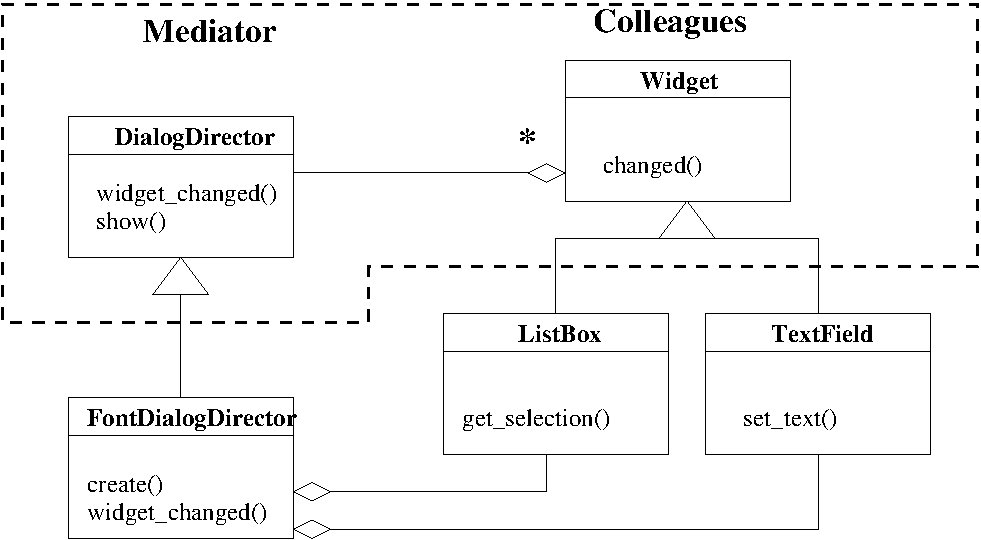
\includegraphics[width=0.9\linewidth]{uml/xfig/mediator}
\end{center}
\includegraphics[width=\linewidth]{uml/xfig/mediator-seq}
\newpage
\section{Adapter}
converts the interface of one class to be what another class expects.
Adapter lets classes work together that couldn't otherwise because of incompatible
interfaces.
\begin{center}
\includegraphics[width=0.75\linewidth]{uml/xfig/pushb-adapter}
\end{center}
%\href{http://www.tutorialspoint.com/design_pattern/design_pattern_quick_guide.htm}
%  {www.tutorialspoint.com/design\_pattern/design\_pattern\_quick\_guide.htm}
\newslide
\begin{lstlisting}[language=java]
public class AdapterDemo {
  public AdapterDemo() {
    Process process = new Process();
    Button button = new Button("Press me");
    button.addActionListener(new Adapter(process) );
    ..
  }
}
\end{lstlisting}
\newslide
\begin{lstlisting}[language=java]
public class Adapter implements ActionListener {
  Process process;

  public Adpater( Process adaptee ){
    process=adaptee;
  }
  public void actionPerformed(ActionEvent e) {
    process.doOperation();
  }
}
\end{lstlisting}
\newslide
Oder etwas kompakter:
\begin{lstlisting}[language=java]
public class AdapterDemo {
  public AdapterDemo() {
    Button button = new Button("Press me");
    button.addActionListener(new ActionListener() {
      public void actionPerformed(ActionEvent e) {
        doOperation();
      }
    });
  }
  public void doOperation() { ... }
}
\end{lstlisting}

\section{Exercise}
\begin{enumerate}
\item Modify the following class in a way that only one
object could exist:
\begin{lstlisting}
public class Storage {
  private int value;

  public void setValue(int value) {
    this.value = value;
  }

  public int getValue() {
    return value;
  }
}
\end{lstlisting}
\end{enumerate}
